\subsection{Additional Figures}
\label{app:additional_figures}
\label{app:extra}
\label{app:lawnmower}

Figures that support the main body but were moved here to keep the results section readable.
All are reproducible from the scripts in \texttt{src/agents/dqn/dqn\_evaluation\_results/}
using the data in \texttt{baseline\_results/}.

\subsection*{Training Convergence}

\begin{figure}[H]
    \centering
    \begin{subfigure}[b]{0.48\textwidth}
        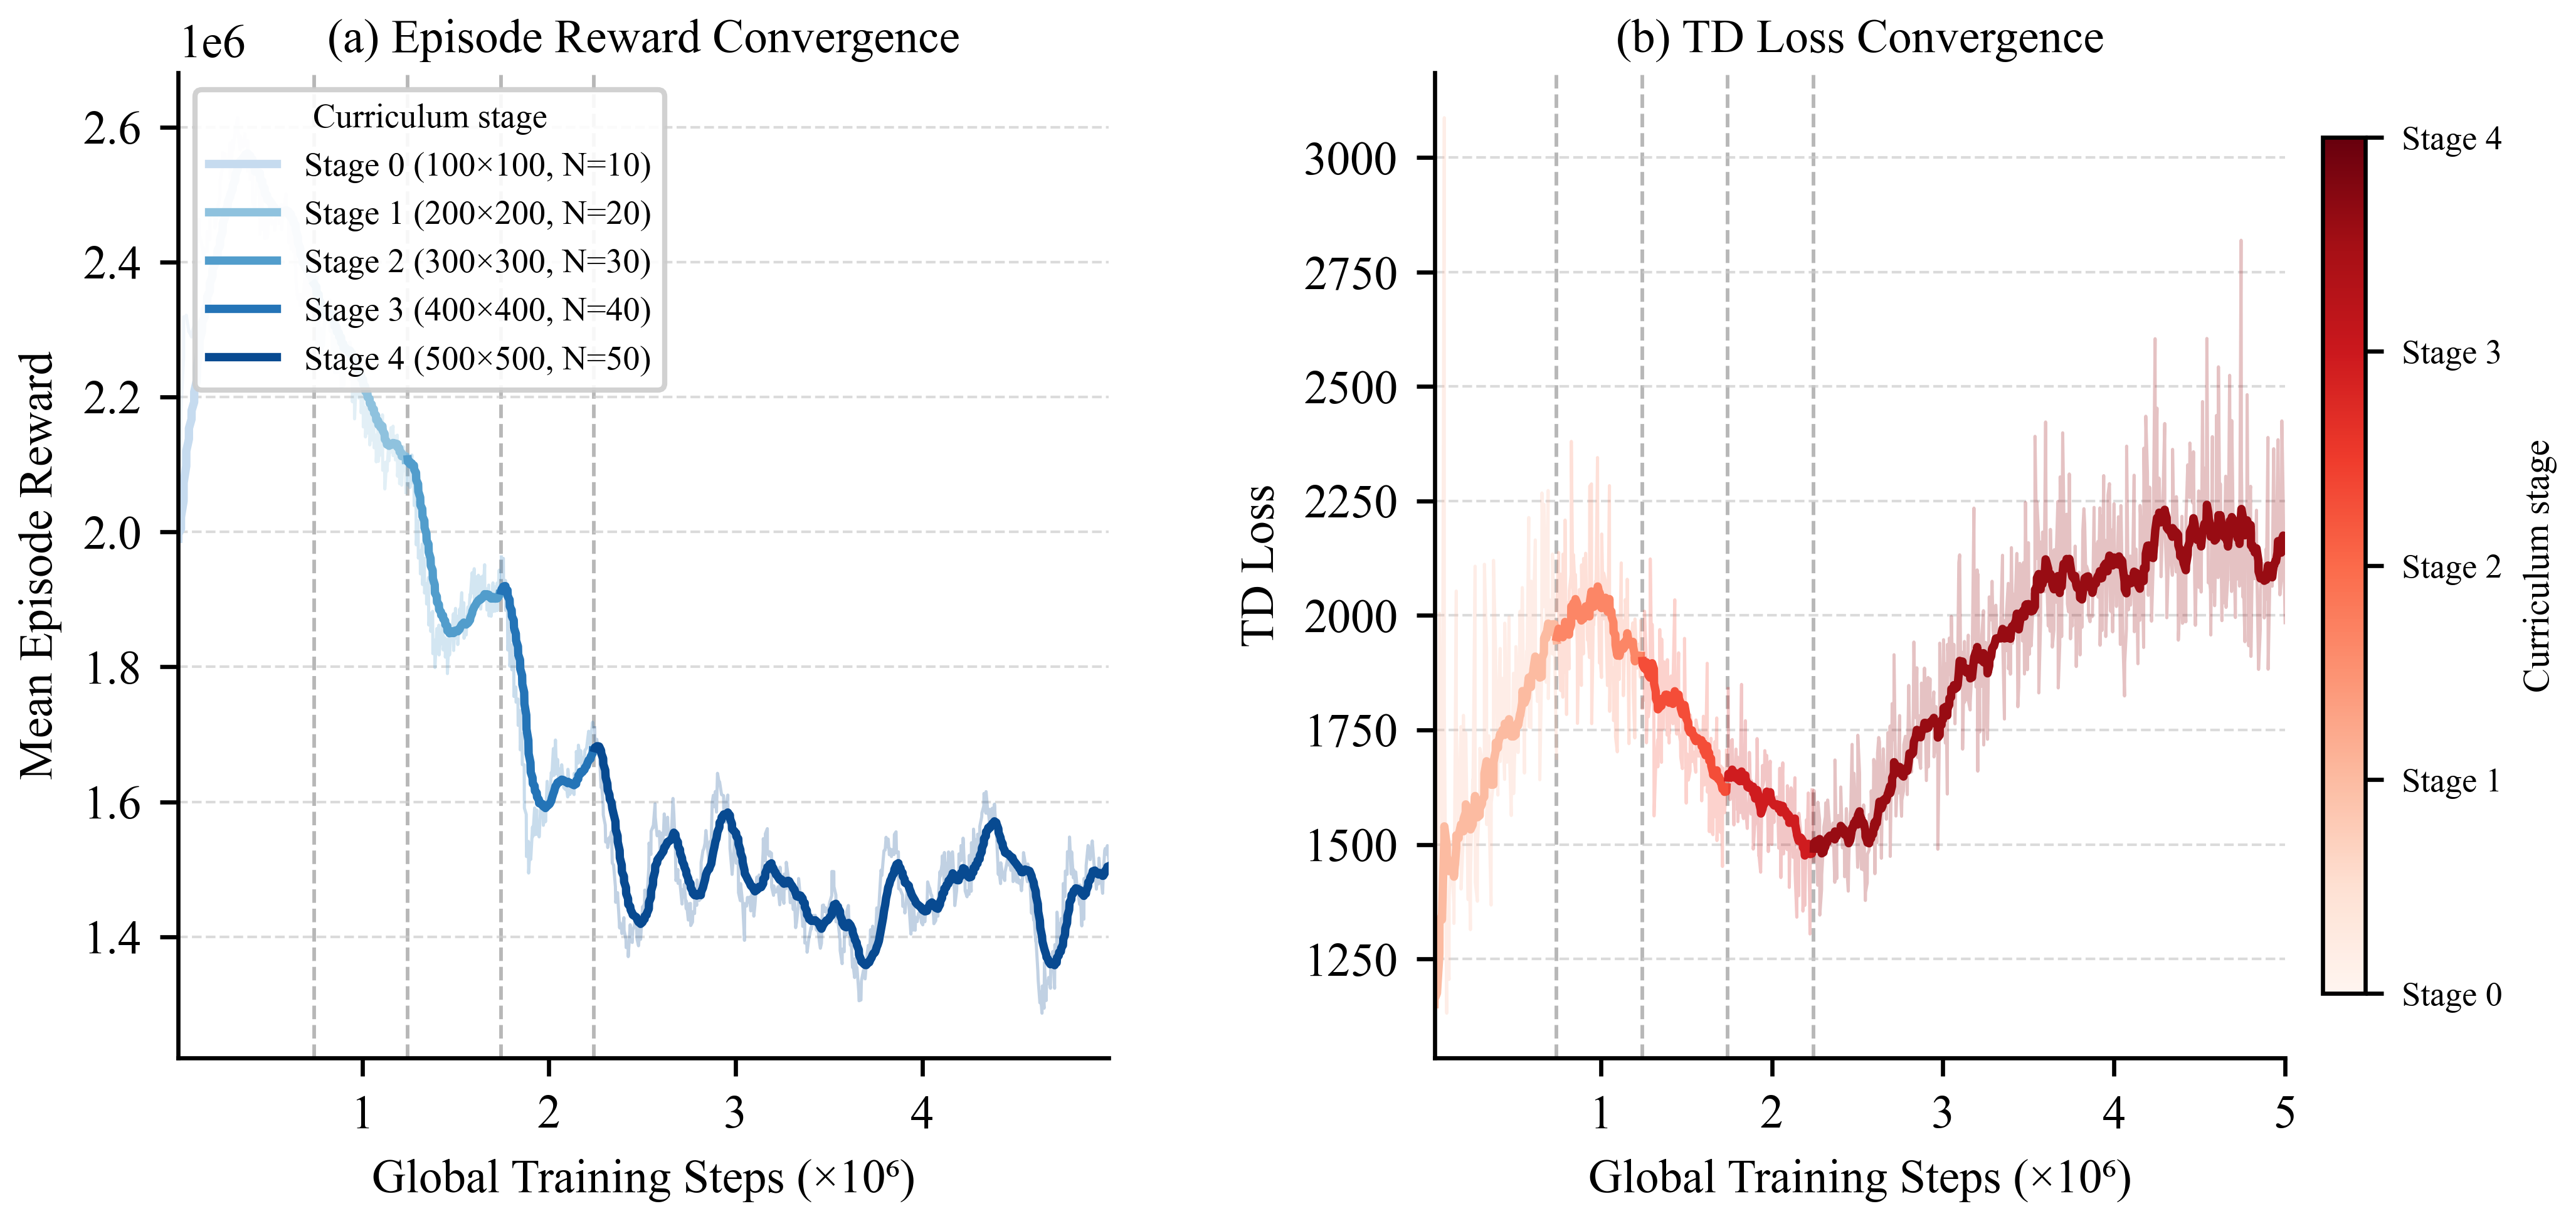
\includegraphics[width=\textwidth]{../src/agents/dqn/dqn_evaluation_results/baseline_results/training_convergence.png}
        \caption{DQN (flat MLP) training.}
    \end{subfigure}
    \hfill
    \begin{subfigure}[b]{0.48\textwidth}
        \includegraphics[width=\textwidth]{../src/agents/dqn/dqn_evaluation_results/baseline_results/relational_convergence.png}
        \caption{Relational RL (PPO) training.}
    \end{subfigure}
    \caption{Training convergence curves for the two learned policies.
    Both reach the curriculum's final stage under the same
    domain-randomised distribution.}
    \label{fig:training_convergence}
\end{figure}

\subsection*{Ablation Study}

\begin{figure}[H]
    \centering
    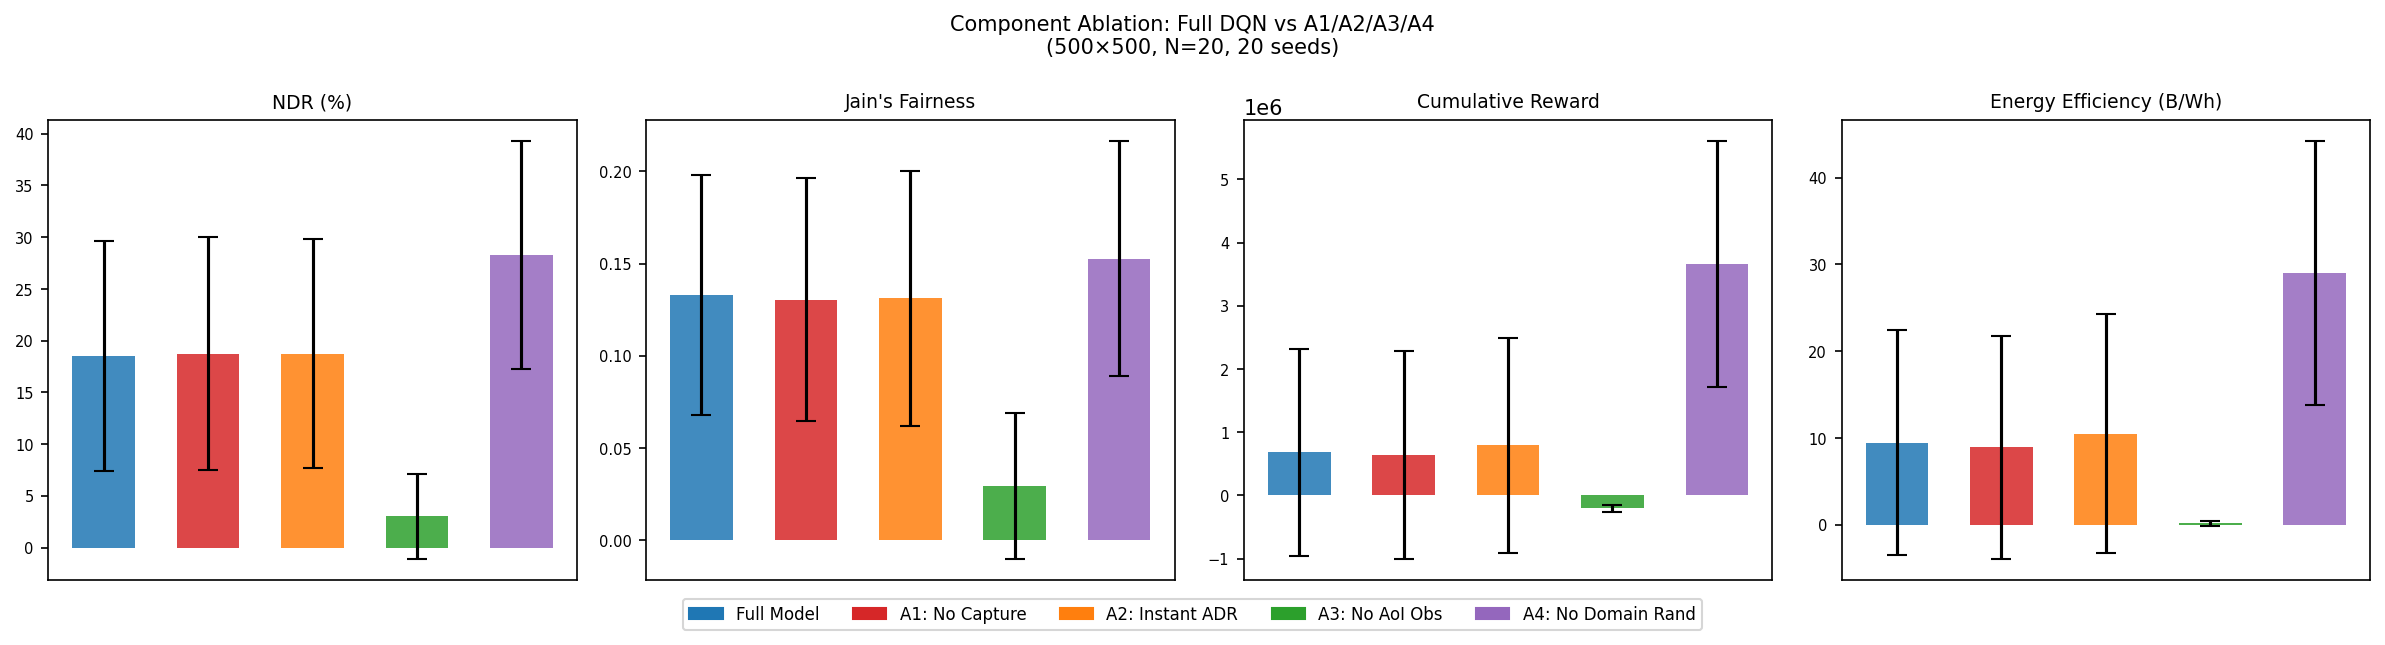
\includegraphics[width=0.92\textwidth]{../src/agents/dqn/dqn_evaluation_results/baseline_results/ablation_comparison.png}
    \caption{Component ablation bars. Full Model versus the four
    ablation conditions (Capture Effect removed, instant ADR, AoI
    zeroed, fixed environment) across cumulative reward, NDR, Jain's
    fairness index, and energy efficiency. Regenerable from
    \texttt{ablation\_study.py}.}
    \label{fig:ablation_bars}
\end{figure}

\subsection*{Multi-Seed Pareto and Radar Views}

\begin{figure}[H]
    \centering
    \begin{subfigure}[b]{0.48\textwidth}
        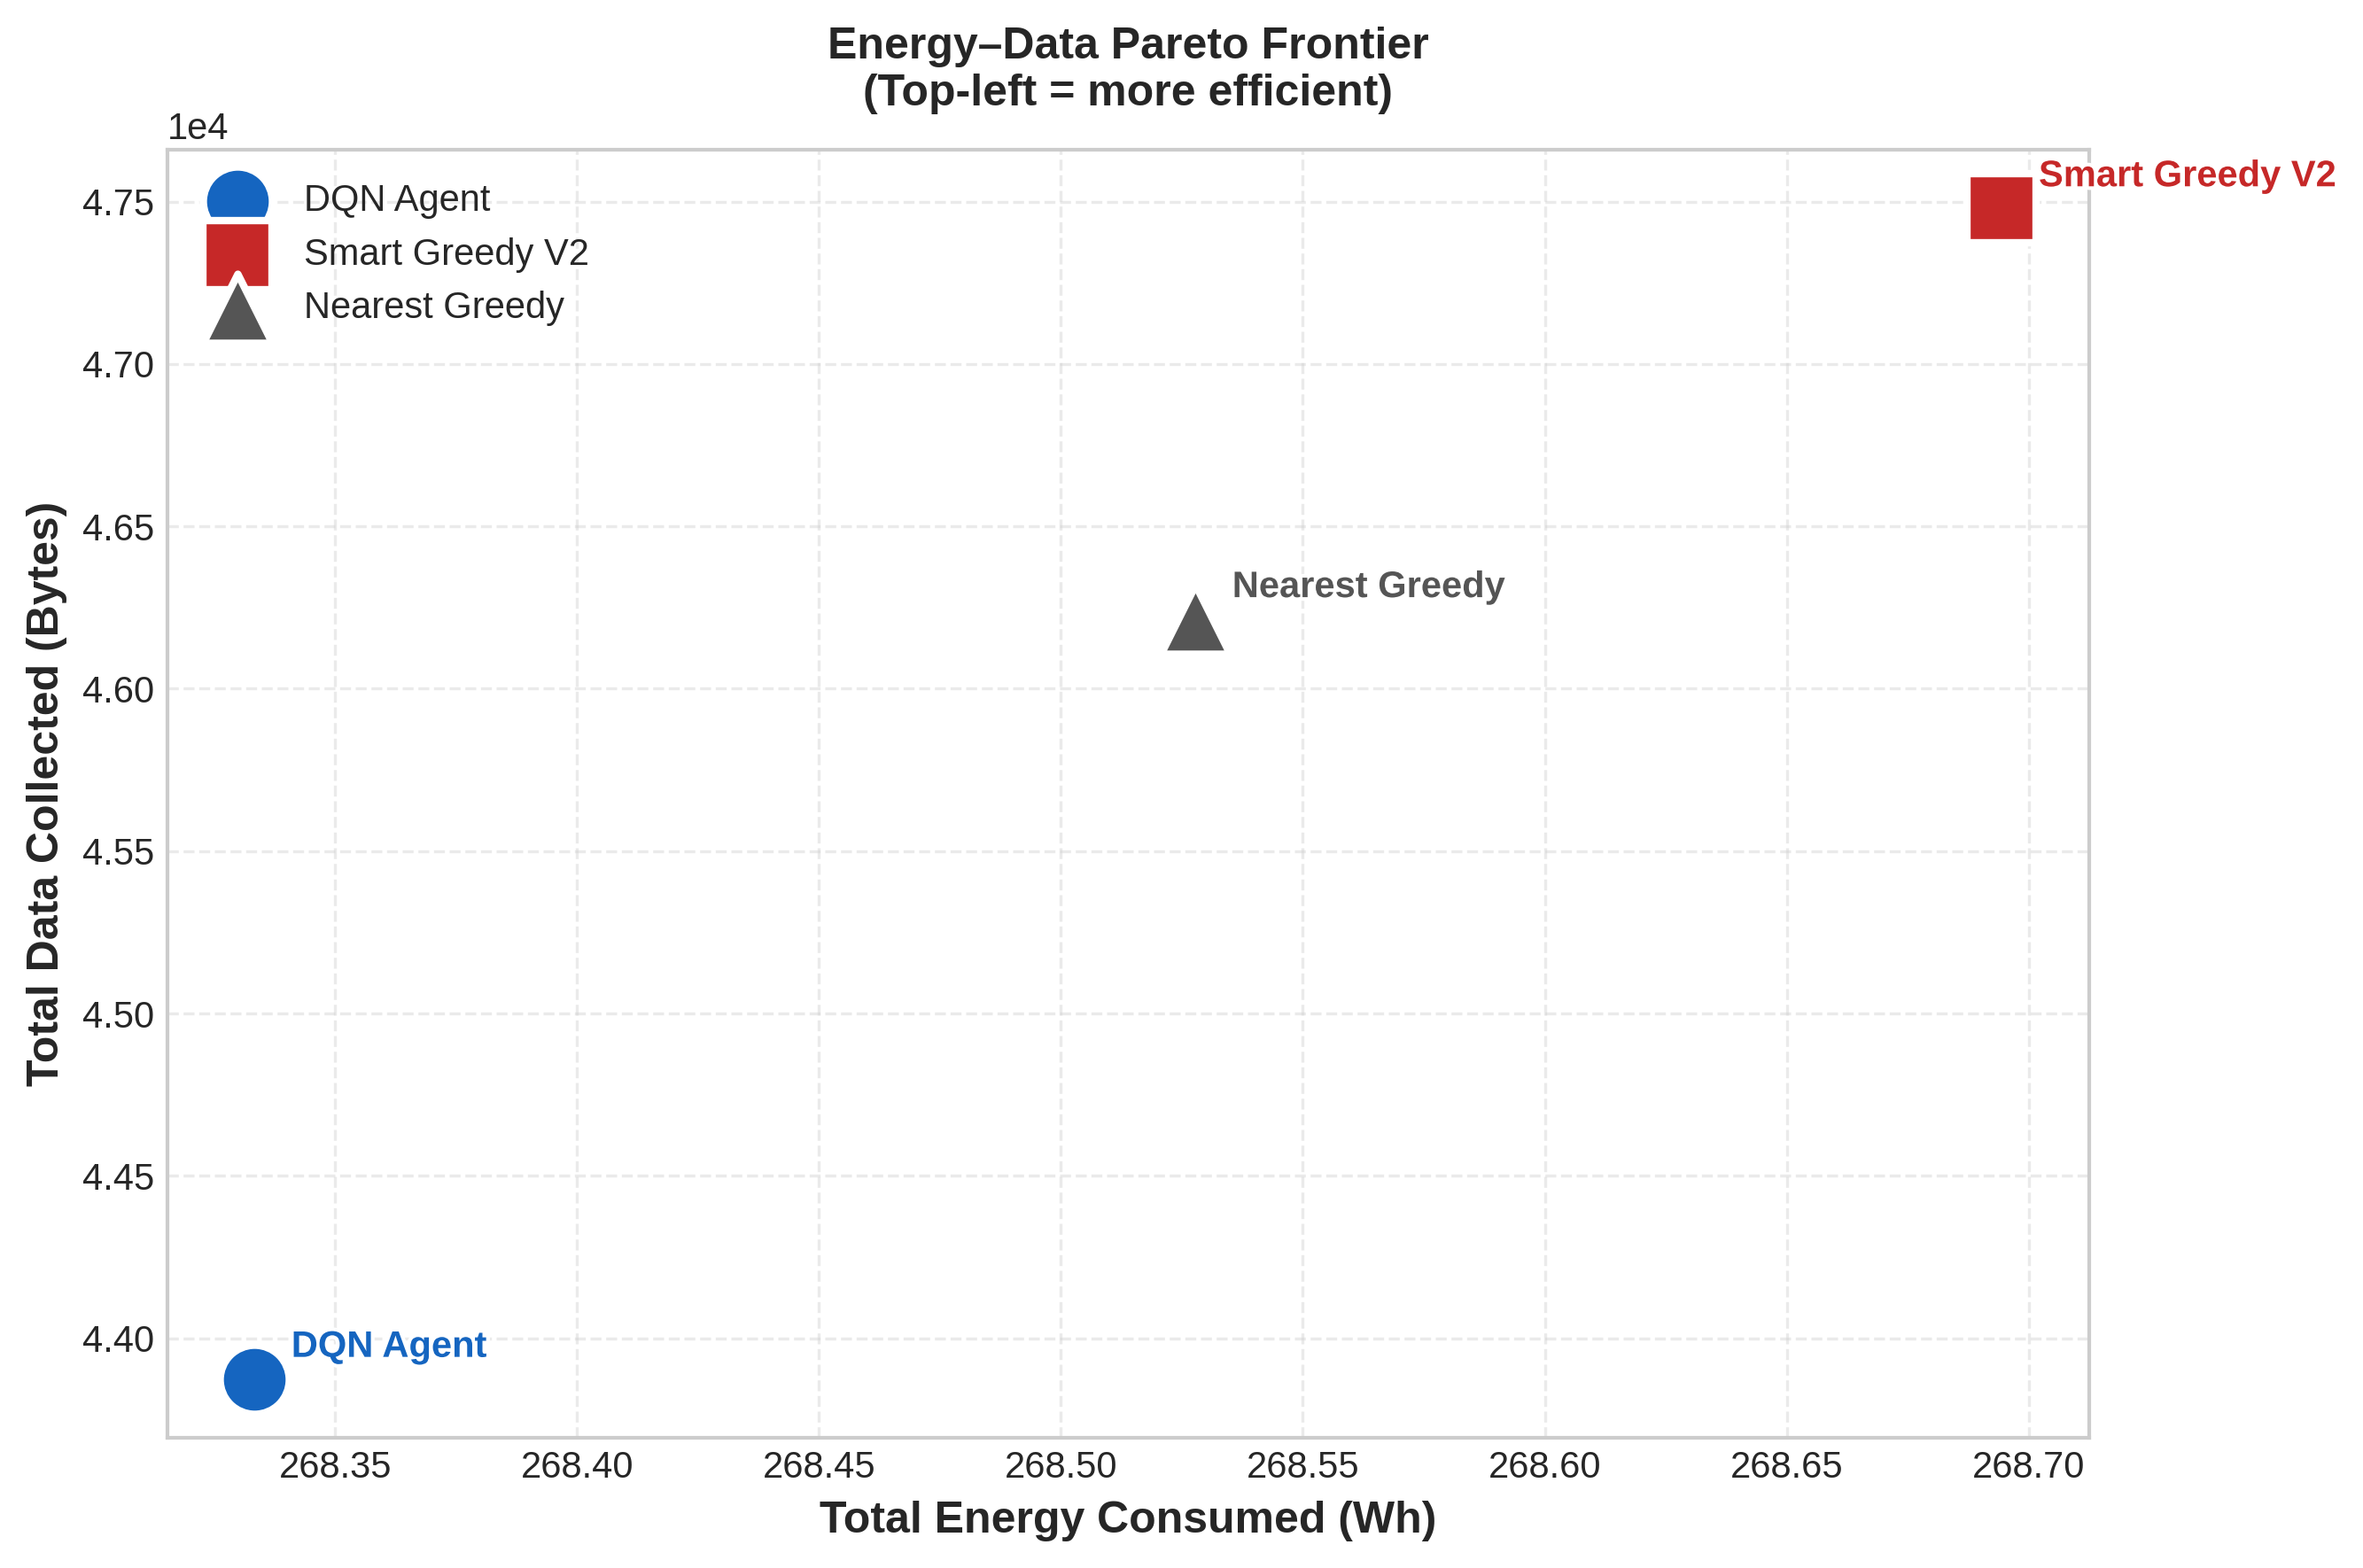
\includegraphics[width=\textwidth]{../src/agents/dqn/dqn_evaluation_results/baseline_results/pareto_scatter.png}
        \caption{Reward vs energy efficiency.}
    \end{subfigure}
    \hfill
    \begin{subfigure}[b]{0.48\textwidth}
        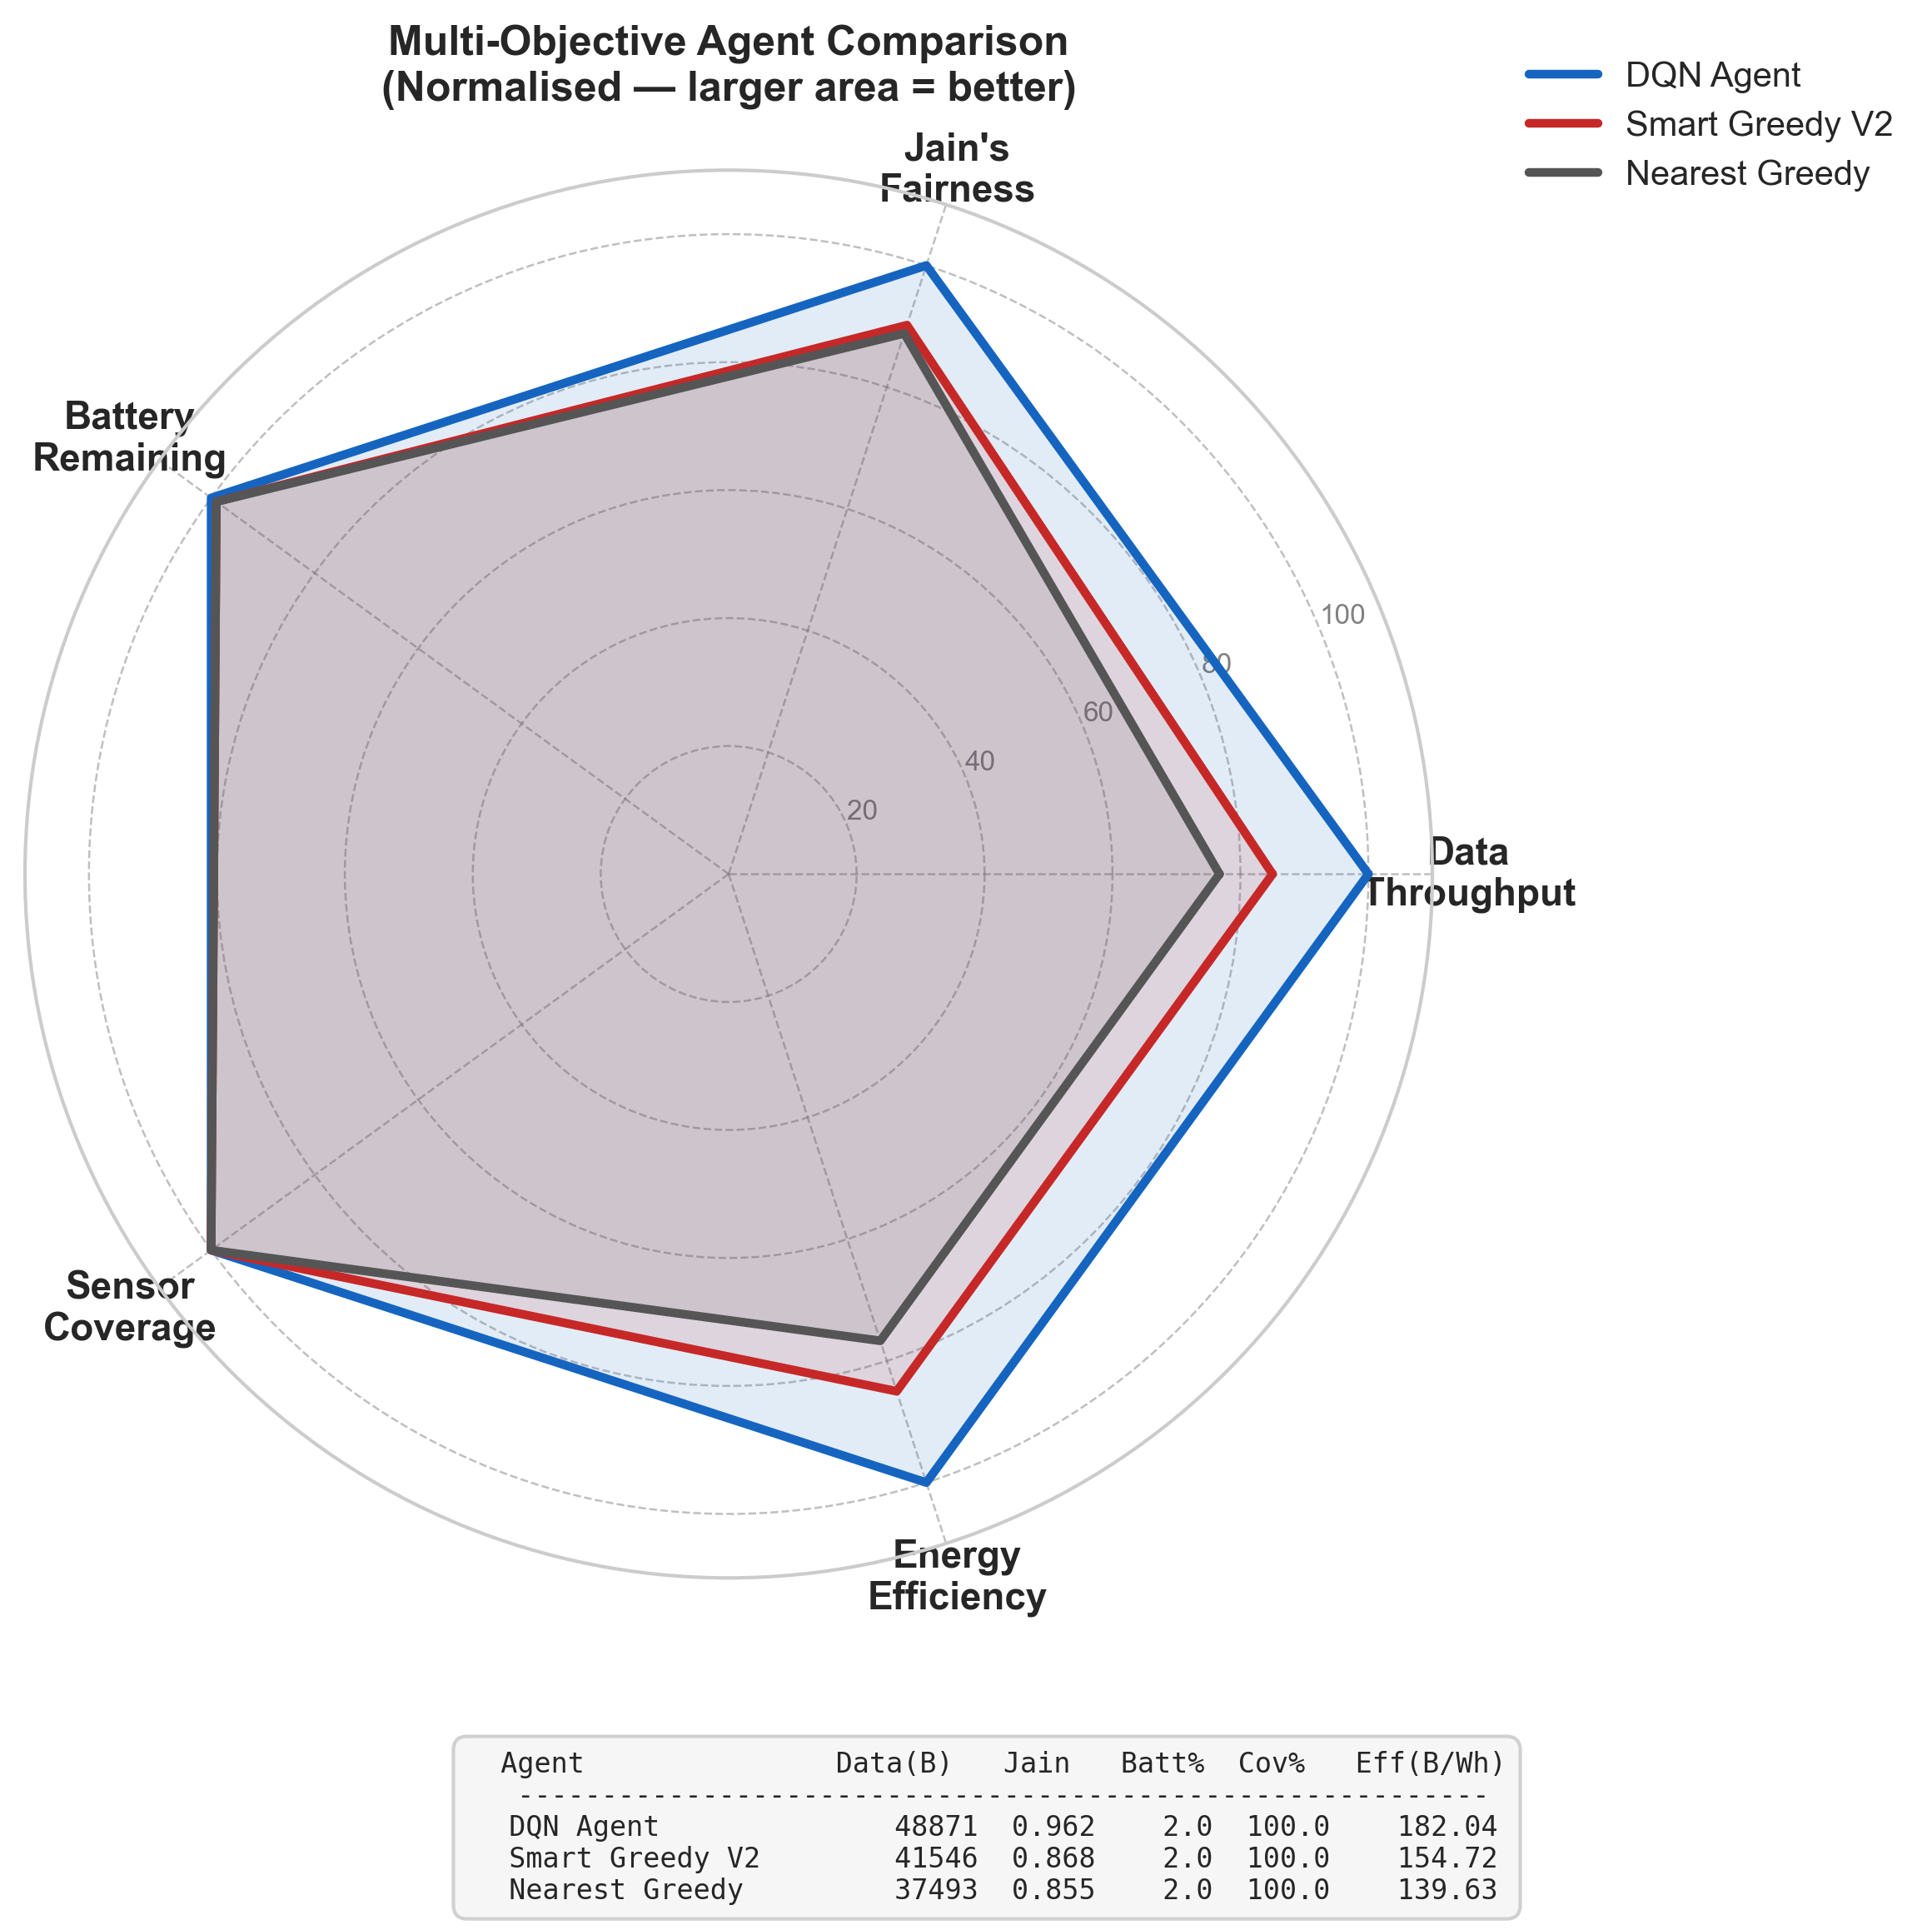
\includegraphics[width=\textwidth]{../src/agents/dqn/dqn_evaluation_results/baseline_results/radar_chart.png}
        \caption{Multi-metric radar.}
    \end{subfigure}
    \caption{The same five-condition scalability data from
    Figure~\ref{fig:scalability_combined}, plotted as a Pareto scatter
    (reward vs energy efficiency) and a multi-metric radar.
    Same 50-seed results, different layout.}
    \label{fig:pareto_radar}
\end{figure}

\subsection*{Fairness Heatmap}

\begin{figure}[H]
    \centering
    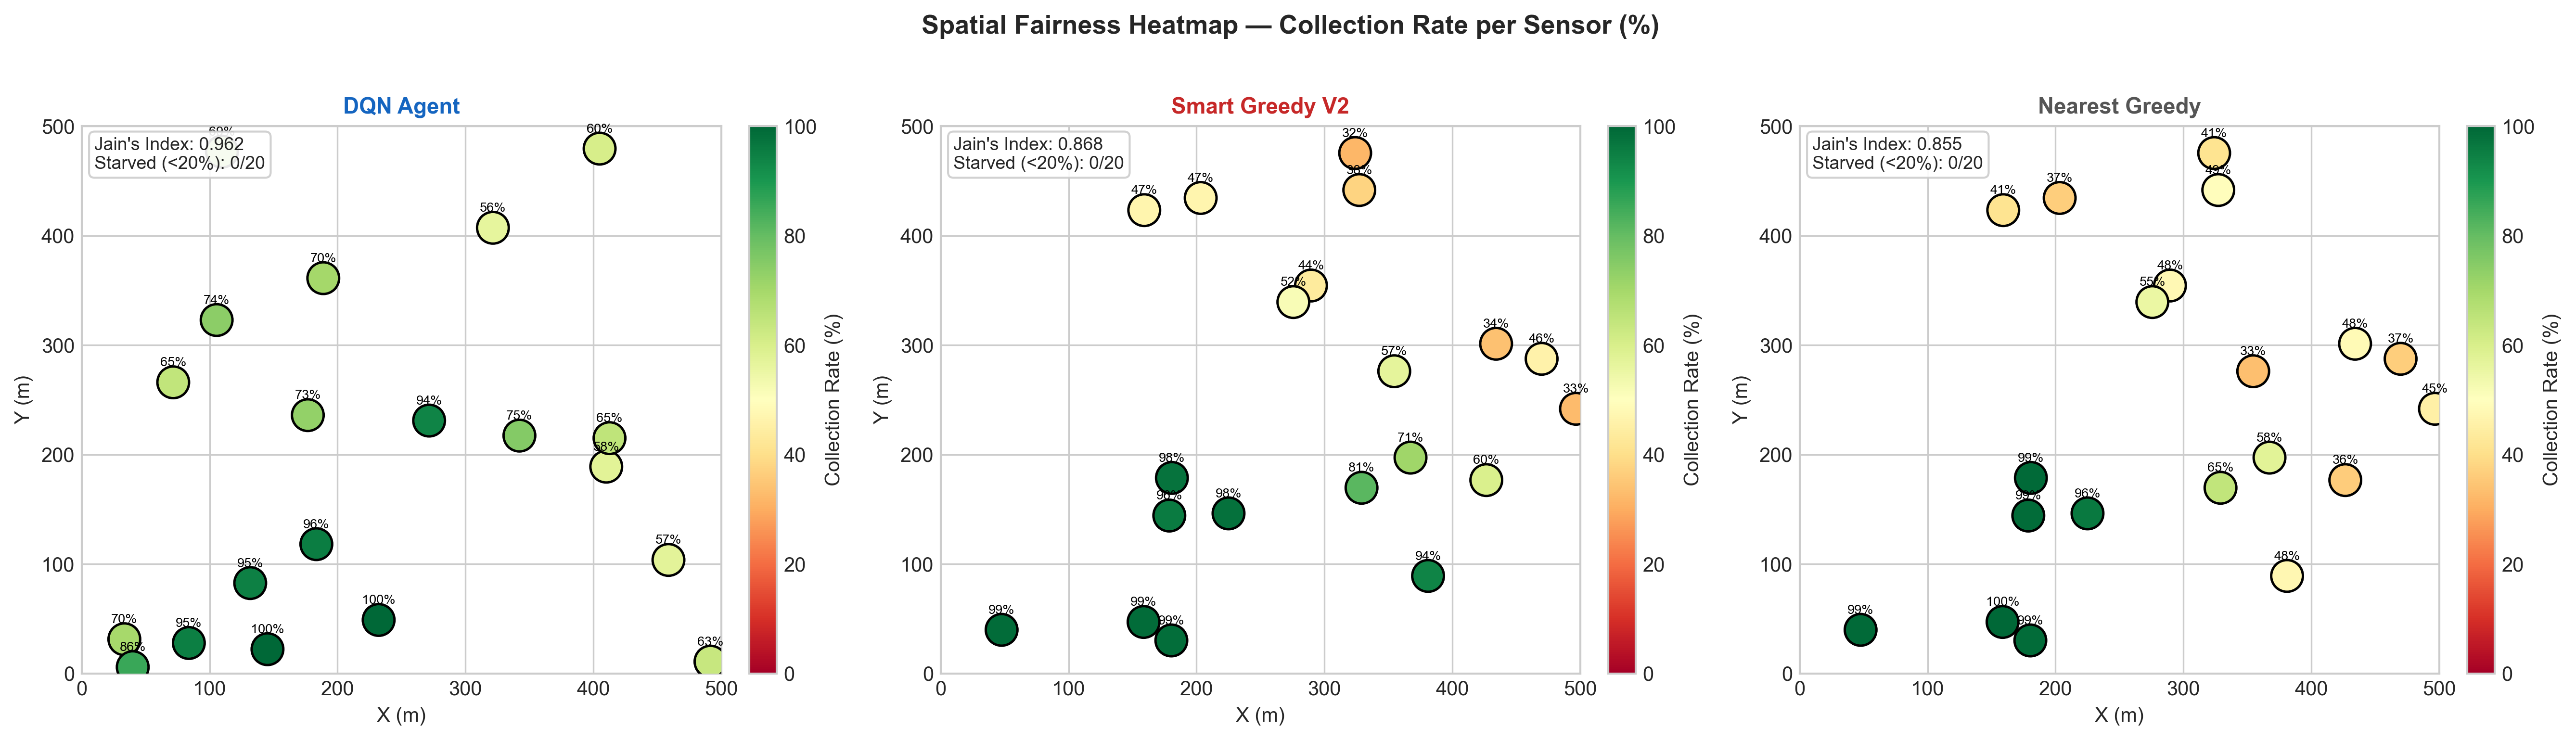
\includegraphics[width=0.85\textwidth]{../src/agents/dqn/dqn_evaluation_results/baseline_results/fairness_heatmap.png}
    \caption{Per-sensor collection fairness heatmap (rows: sensors,
    columns: agents). Darker cells indicate higher fraction of the
    sensor's total data successfully collected.}
    \label{fig:fairness_heatmap}
\end{figure}

\subsection*{Lawnmower Indicative Results}

The Lawnmower baseline was run at 5 seeds, not 50; per-episode reward
and per-metric traces are in \texttt{baseline\_results/lawnmower\_results.csv}.
At $200{\times}200$, $N{=}50$ it achieves $98\%$ coverage with cumulative
reward roughly $78\%$ of the DQN's on the matched seed. It is a
coverage-only indicator and is not included in the statistical comparisons
in the main body.
